%
% Modified by Megan Patnott
% Last Change: Jan 18, 2013
%
%%%%%%%%%%%%%%%%%%%%%%%%%%%%%%%%%%%%%%%%%%%%%%%%%%%%%%%%%%%%%%%%%%%%%%%%
%
% Modified by Sameer Vijay
% Last Change: Tue Jul 26 2005 13:00 CEST
%
%%%%%%%%%%%%%%%%%%%%%%%%%%%%%%%%%%%%%%%%%%%%%%%%%%%%%%%%%%%%%%%%%%%%%%%%
%
% Sample Notre Dame Thesis/Dissertation
% Using Donald Peterson's ndthesis classfile
%
% Written by Jeff Squyres and Don Peterson
%
% Provided by the Information Technology Committee of
%   the Graduate Student Union
%   http://www.gsu.nd.edu/
%
% Nothing in this document is serious except the format.  :-)
%
% If you have any suggestions, comments, questions, please send e-mail
% to: ndthesis@gsu.nd.edu
%
%%%%%%%%%%%%%%%%%%%%%%%%%%%%%%%%%%%%%%%%%%%%%%%%%%%%%%%%%%%%%%%%%%%%%%%%


%
% Chapter 5
%


\chapter{R-matrix analysis}
\label{chap: r-matrix}

An $R$-matrix analysis was performed to analyze the effects of the new lifetime and cross sections measurements described earlier. Such an analysis can be used to transform the cross sections into $S$ factors, which removes the Coulomb repulsion component of the cross-section and provides higher fidelity extrapolations to astrophysical energies. The $^{14}$N$(p,\gamma)^{15}$O system is ideal for $R$-matrix analysis because it is comprised of light nuclei with a discrete level structure at relatively low energies. While there are many programs available for performing $R$-matrix fits, we use the \texttt{AZURE2} code \cite{Azuma2010}, which was also used for similar, previous measurements \cite{Li2016}. 

\section{Impact of new lifetimes}
\label{sec: lifetime fit}

Following the analysis of \citet{Li2016}, the width of the 6.79 MeV state in $^{15}$O  was previously the largest source of uncertainty in the low-energy extrapolations of the cross section. A set of $R$-matrix fits was employed to explore the impact of our newly measured lifetimes. To isolate the effects of our measurement, we selected discrete lifetimes within our uncertainty range for the lifetime of the 6.79 MeV state in $^{15}$O, converted them to their equivalent radiative width, and used those level width values throughout the fit and extrapolation. This collection of fits, therefore, serves primarily as an illustration of the ways in which these new lifetime measurements impact the low energy extrapolations of the cross section.

In the fits presented here, the information about the levels was taken from  \citet{Ajzenberg-Selove1991} or \citet{Daigle2016} where updated. A channel radius of 5.5 fm was adopted for this work, which matches the analyses done by Refs.~\cite{Adelberger2011, Li2016, Wagner2018}. Information about the levels and their parameters as used in \texttt{AZURE2} are contained in Table~\ref{table: fitParams}. 


\begin{table*}[]
\thisfloatpagestyle{plain}
\caption{$R$-MATRIX FIT PARAMETERS FOR EXPLORING THE IMPACT OF NEWLY MEASURED LIFETIMES}
\begin{center}
\begin{threeparttable}
\begin{tabular}{c  c  c  c  c  c  c}
\toprule
$E_x$ (Ref.~\cite{Ajzenberg-Selove1991}) &   $E_x$ (fit) & $J^\pi$ & Channel & l & s & ANC (fm$^{-1/2}$) / $\Gamma$ (eV)\\ 
\midrule
0.0 & 0.0	& 1/2$^-$ &	$^{14}$N+p &	1&	1/2&	{0.23}\\
	&	&	    &    $^{14}$N+p &	1&	3/2&	{7.4} \\
%5.183(1) & \textbf{5.183}&	1/2$^+$&	$^{14}$N+p&	0&	1/2&	\textbf{0.33}\\
%	&	&		    &$^{15}$O+$\gamma_{0.00}$  &	E1&	1/2&	\textbf{0.0784}\\
%5.2409(3) & \textbf{5.2409}&	5/2$^+$&	$^{14}$N+p &	2&	1/2&	\textbf{0.23}\\
%                &	&		  & $^{14}$N+p &	2&	3/2&	\textbf{0.24}\\
%	 			&	&	 &$^{15}$O+$\gamma_{0.00}$	&M2&	1/2&	\textbf{0.0002}\\
%6.1763(17) & \textbf{6.1763}&	3/2$^-$& $^{14}$N+p &	1&	1/2&	\textbf{0.47}\\
%				&	&	& $^{14}$N+p	&1	&3/2	&\textbf{0.53}\\
%				&	&	&$^{15}$O+$\gamma_{0.00}$	&M1	&1/2&	\textbf{0.865}\\
6.7931(17) & {6.7931}&	3/2$^+$ & $^{14}$N+p &	0&	3/2&	{4.75}\\
	&	&	     &  $^{15}$O+$\gamma_{0.00}$	&  E1  &	1/2&	\textbf{2.50$^{\text{a}}$}\\
%	& &       &  $^{15}$O+$\gamma_{6.17}$	&  E1  &	3/2&{-0.002}\\
%6.8594(9) & \textbf{6.8594}&	5/2$^+$&	$^{14}$N+p&	2&	1/2&\textbf{0.39}\\
%	&		&    &     $^{14}$N+p&	2&	3/2&	\textbf{0.42}\\
%	&		&    &     $^{15}$O+$\gamma_{5.24}$&	M1&	5/2&	\textbf{0.04}\\
%7.2759(6) & \textbf{7.2759}&	7/2$^+$&	$^{14}$N+p &	2&	3/2&	\textbf{1541}\\
%	&		&    &     $^{15}$O+$\gamma_{5.24}$&	M1&	5/2&	\textbf{0.00099}\\
\hline
%7.5565(4) & 7.5563	&	1/2$^+$	&	$^{14}$N+p	&	0	&	1/2	&	\textbf{1.0$\times$10$^3$}	\\
%	&	&	&	$^{15}$O+$\gamma_{0.00}$	&	E1	&	1/2	&	\textbf{0.61$\times$10$^{-3}$}\\
%	&	&	&	$^{15}$O+$\gamma_{6.79}$	&	M1	&	3/2	&	\textbf{8.22$\times$10$^{-3}$}\\
%	&	&	&	$^{15}$O+$\gamma_{5.18}$	&	M1	&	1/2	&	\textbf{0.006}\\
%	&	&	&	$^{15}$O+$\gamma_{6.17}$	&	E1	&	3/2	&	\textbf{0.0254}\\
8.2840(5)& \textbf{8.2848}&	3/2$^+$	&	$^{14}$N+p	&	2	&	1/2	&	{-92.2}\\
	&	&	&	$^{14}$N+p	&	0	&	3/2	&	\textbf{4.013$\times$10$^3$}\\
	&	&	&	$^{14}$N+p	&	2	&	3/2	&	{-509}\\
	&	&	&	$^{15}$O+$\gamma_{0.00}$	&	E1	&	1/2	&	\textbf{0.244}\\
%	&	&	&	$^{15}$O+$\gamma_{5.18}$	&	M1	&	1/2	&	{0.01}\\
%	&	&	&	$^{15}$O+$\gamma_{5.24}$	&	M1	&	5/2	&	{0.2}\\
%	&	&	&	$^{15}$O+$\gamma_{6.17}$	&	E1	&	3/2	&	{-4$\times$10$^{-3}$}\\
%	&	&	&	$^{15}$O+$\gamma_{6.86}$	&	M1	&	5/2	&	{0.01}\\
%8.743(6) & \textbf{8.7502}&	1/2$^+$	&	$^{14}$N+p	&	0	&	1/2	&	\textbf{35.726$\times$10$^3$}\\
%	&	&	&	$^{15}$O+$\gamma_{5.18}$	&	M1	&	1/2	&	\textbf{-0.2}\\
%	&	&	&	$^{15}$O+$\gamma_{6.17}$	&	E1	&	3/2	&	\textbf{0.0827}\\
%8.922(2) & \textbf{8.9219}&	5/2$^+$	&	$^{14}$N+p	&	2	&	3/2	&	\textbf{3.8$\times$10$^3$}\\
%	&	&	&	$^{15}$O+$\gamma_{6.79}$	&	M1	&	3/2	&	\textbf{0.003}\\
8.9821(17) & {8.98}&	5/2$^-$	&	$^{14}$N+p	&	1	&	3/2	&	\textbf{-5.872$\times$10$^3$}\\
	&	&	&	$^{15}$O+$\gamma_{0.00}$	&	E2	&	1/2	&	\textbf{-0.303}\\
	&	&	&	$^{15}$O+$\gamma_{6.79}$	&	E1	&	3/2	&	{-0.001}\\
9.484(8) & \textbf{9.488}&	3/2$^+$	&	$^{14}$N+p	&	2	&	1/2	&	{77.69$\times$10$^3$}	\\
	&	&	&	$^{14}$N+p	&	0	&	3/2	&	\textbf{126.685$\times$10$^3$}	\\
	&	&	&	$^{14}$N+p	&	2	&	3/2	&	{-7.822$\times$10$^3$}\\
	&	&	&	$^{15}$O+$\gamma_{0.00}$	&	E1	&	1/2	&	\textbf{6.92}\\
%	&	&	&	$^{15}$O+$\gamma_{6.86}$	&	M1	&	5/2	&	{0.2}\\
9.488(3) & {9.4905}&	5/2$^-$	&	$^{14}$N+p	&	3	&	1/2	&	{0.979$\times$10$^3$}\\
	&	&	&	$^{14}$N+p	&	1	&	3/2	&	{-6.576$\times$10$^3$}\\
	&	&	&	$^{14}$N+p	&	3	&	3/2	&	{-0.985$\times$10$^3$}\\
	&	&	&	$^{15}$O+$\gamma_{0.00}$	&	E2	&	1/2	&	\textbf{-0.307}\\
	&	&	&	$^{15}$O+$\gamma_{6.79}$	&	E1	&	3/2	&	{-0.0123}\\
9.609(2) & {9.6075}&	3/2$^-$	&	$^{14}$N+p	&	1	&	3/2	&	\textbf{-13.821$\times$10$^3$}\\
	&	&	&	$^{15}$O+$\gamma_{0.00}$	&	M1	&	1/2	&	\textbf{1.24}\\
     &	&	&	$^{15}$O+$\gamma_{6.79}$	&	E1	&	3/2	&	{-0.044}\\
%	&	&	&	$^{15}$O+$\gamma_{5.24}$	&	E1	&	5/2	&	{0.095}\\
%10.2817 & \textbf{10.2817}	&	5/2$^+$	&	$^{14}$N+p	&	2	&	3/2	&	\textbf{17.292$\times$10$^3$}\\
%	&	&	&	$^{15}$O+$\gamma_{6.79}$	&	M1	&	3/2	&	\textbf{0.2}\\	
%	&	&	&	$^{15}$O+$\gamma_{6.86}$	&	M1	&	5/2	&	\textbf{-0.4}\\	
%10.480 & \textbf{10.4675}	&	3/2$^-$	&	$^{14}$N+p	&	1	&	1/2	&	\textbf{28.998$\times$10$^3$}\\
%	&	&	&	$^{14}$N+p	&	1	&	3/2	&	\textbf{9.652$\times$10$^3$}\\
%	&	&	&	$^{15}$O+$\gamma_{0.00}$	&	M1	&	1/2	&	\textbf{-0.404}\\	
%	&	&	&	$^{15}$O+$\gamma_{6.79}$	&	E1	&	3/2	&	\textbf{0.1}\\
%	&	&	&	$^{15}$O+$\gamma_{6.86}$	&	E1	&	5/2	&	\textbf{0.1}\\
%10.506 & \textbf{10.5313}&	3/2$^+$	&	$^{14}$N+p	&	0	&	3/2	&	\textbf{205$\times$10$^3$}\\
%	&	&	&	$^{15}$O+$\gamma_{0.00}$	&	E1	&	1/2	&	\textbf{-0.195}\\
%	&	&	&	$^{15}$O+$\gamma_{6.79}$	&	M1	&	3/2	&	\textbf{0.3}\\
%	&	&	&	$^{15}$O+$\gamma_{6.86}$	&	M1	&	5/2	&	\textbf{-0.4}\\
%10.9288 & \textbf{10.9288}&	7/2$^+$	&	$^{14}$N+p	&	2	&	3/2	&	\textbf{56.948$\times$10$^3$}\\
%	&	&	&	$^{15}$O+$\gamma_{6.79}$	&	E2&	3/2	&	\textbf{1}\\
%11.218(3) & 11.217(2)& 3/2$^+$&	$^{14}$N+p	&	0	&	3/2	&	\textbf{40$\times$10$^3$}\\
%	&	&	&	$^{15}$O+$\gamma_{0.00}$	&	E1	&	1/2	& 5.21	\\   	
& {15}	&	3/2$^+$	&	$^{14}$N+p	&	0	&	3/2	&	\textbf{4.722$\times$10$^6$}\\
	&	&	&	$^{15}$O+$\gamma_{0.00}$	&	E1	&	1/2	&	\textbf{327.3}	\\
%& \textbf{15}	&	5/2$^+$	&	$^{14}$N+p	&	2	&	1/2	&	\textbf{1.452$\times$10$^7$}\\
\bottomrule
\end{tabular}
\begin{tablenotes}
\small 
\item Levels used in the \textit{R}-matrix fits. Bold values indicate parameters which were allowed to vary during the fit. The signs on the partial widths and ANCs indicates the relative interferences. The dividing line demarcates the proton separation energy at $E_x$ = 7.2968(5) MeV \cite{Ajzenberg-Selove1991}. Levels where all parameters are fixed are not shown in this table for brevity but were included in the fits. a) Indicates the partial width of the 6.79 MeV state, measured in this experiment to between $\Gamma$ = 0.66 - 3.29 eV. For each individual fit, this width was fixed. However, between each fit, this width was varied to different values within our range to explore how the uncertainty in this measurement affects the low energy extrapolation. These different fits are shown in Fig.\ \ref{fig: rmatrixRange} and are otherwise identical.
\end{tablenotes}
\end{threeparttable}
\label{table: fitParams}
\end{center}
\end{table*}  



The cross-section data utilized in the fitting routine were from measurements at LUNA \cite{Formicola2004, Imbriani2005, Marta2008, Marta2011}, TUNL \cite{Runkle2005}, Bochum \cite{Schroder1987}, and the University of Notre Dame \cite{Li2016}. All of these data sets were left without scaling during the fits. The Bochum data from \citet{Schroder1987} were corrected as detailed in SFII \cite{Adelberger2011}. Additionally, the data used from \citet{Li2016} are a differential cross section taken at 45$\degree$ and are treated as such in the fits. This dataset was scaled by a factor of 4$\pi$ in the plotting only to compare to the angle integrated data. 

Only statistical uncertainties were included in the fitting. The alternative parameterization of \citet{PhysRevC.66.044611} was used. Its two main advantages are that it eliminates the need for boundary conditions and that the fit parameters correspond directly to physical level parameters.



\begin{figure}[h!]
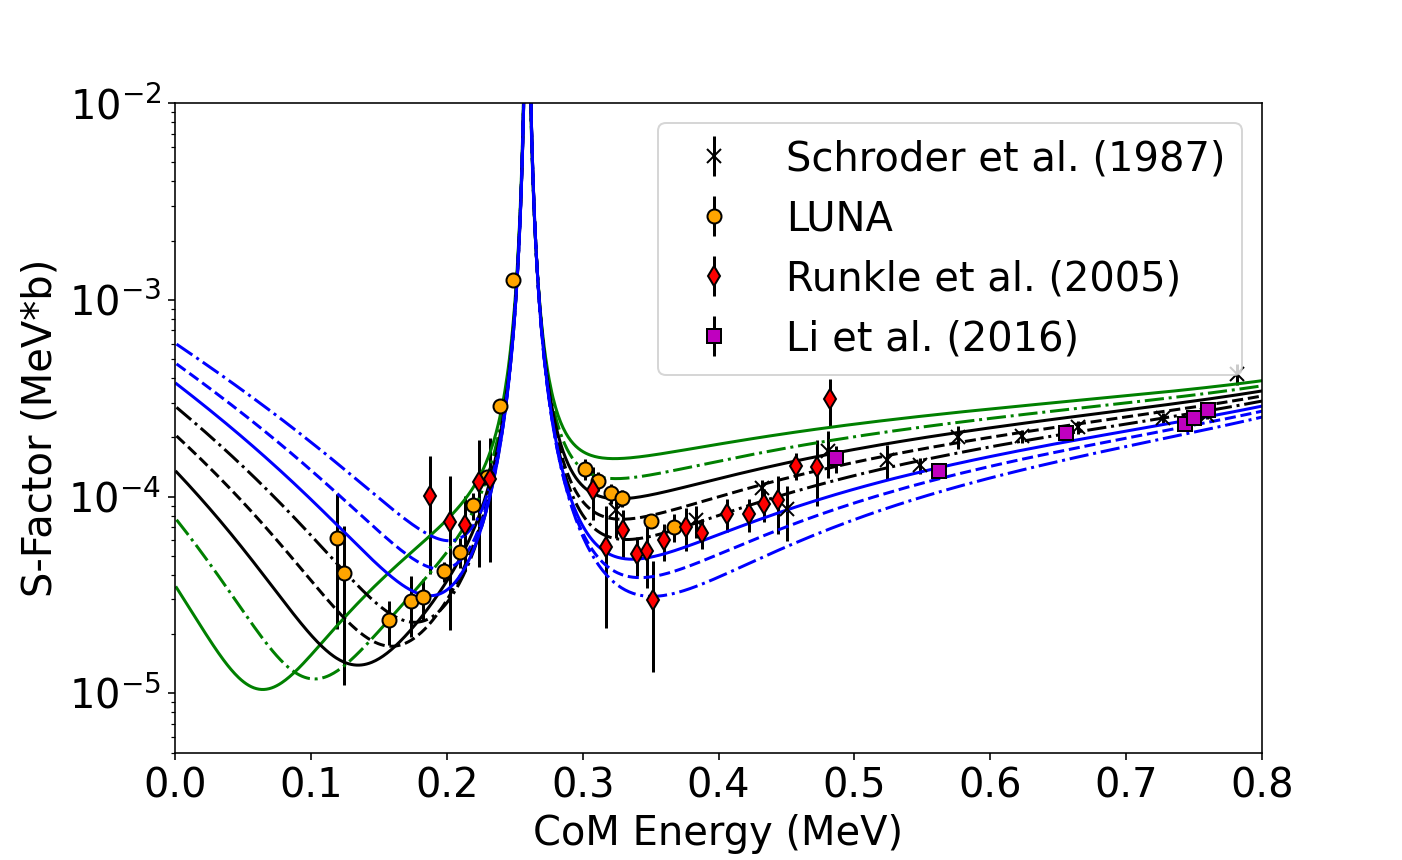
\includegraphics[width=1.0\linewidth]{./figures/lifetimeEffects.png}
\caption{$R$-Matrix fits exploring the uncertainty of our lifetime measurements to the low energy extrapolation. The width of the 6.79 MeV excited state in $^{15}$O is fixed during each fit and changed in each subsequent iteration to another value within our uncertainty range. This clearly shows that even though our lifetime result provides the most stringent limitation on the lifetime of this state, it still has an outsized effect on the low energy behavior of this reaction. The Schr{\"{o}}der et al.~data are from \cite{Schroder1987}, while the LUNA data represents the measurements \cite{Formicola2004, Imbriani2005, Marta2008, Marta2011}, the Runkle et al.~data are from \cite{Runkle2005}, and the Li et al.~data are from \cite{Li2016}. Of these, the data used from \citet{Li2016} are differential and were treated as such in the fitting but scaled up by 4$\pi$ for plotting purposes.}
\label{fig: rmatrixRange}
\end{figure}


\begin{figure}[h!]
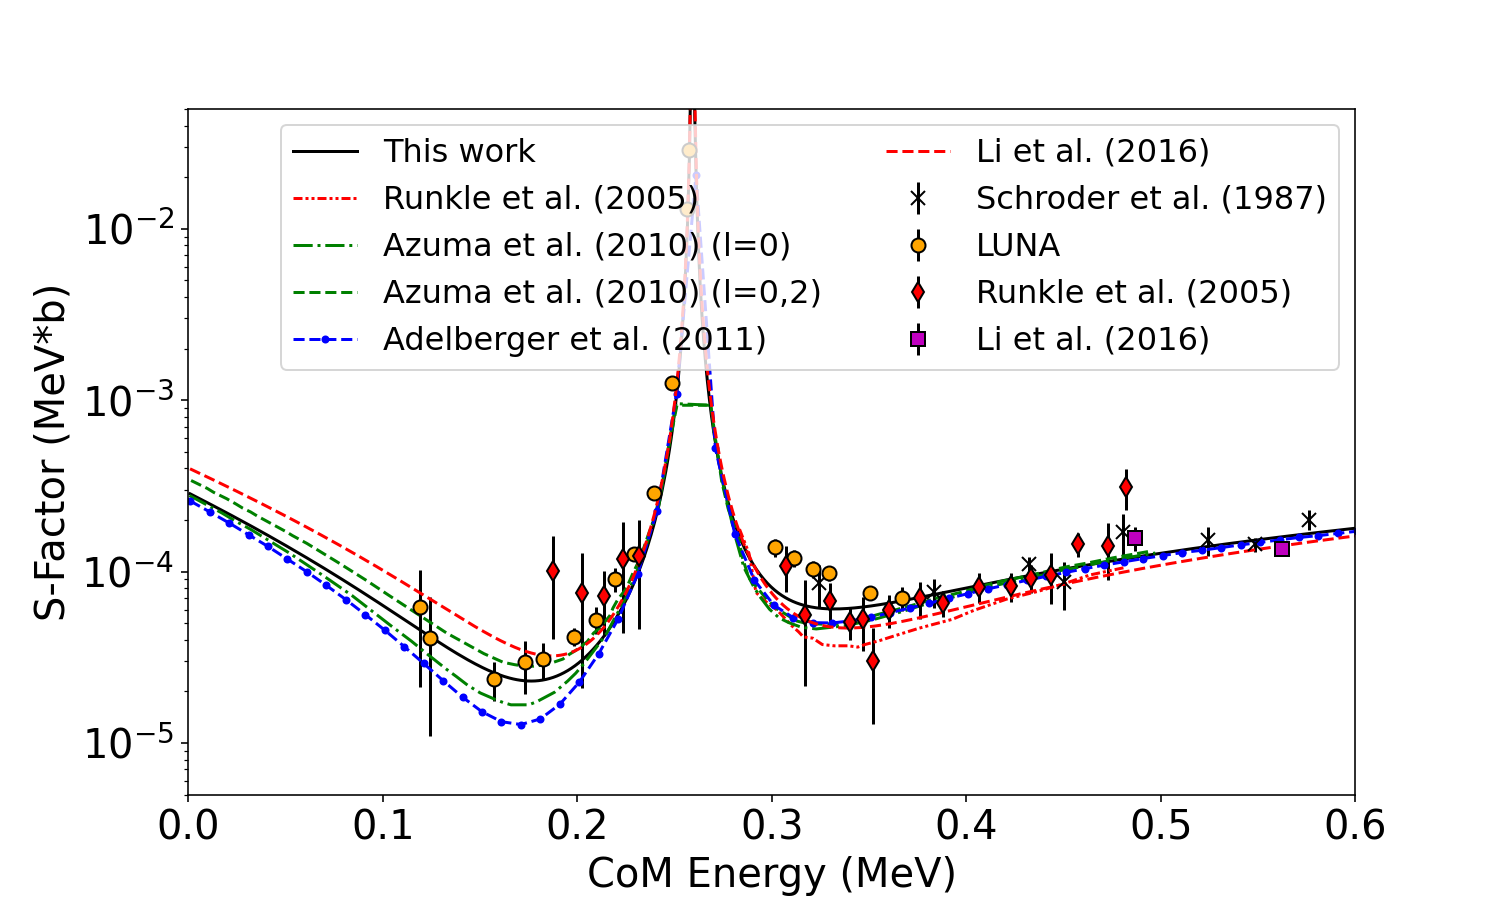
\includegraphics[width=1.0\linewidth]{./figures/bestFits.png}
\caption{$R$-matrix fits comparing our best fit with the lifetimes to those performed in previous works. Our fit used a lifetime value for the 6.79 MeV excited state in $^{15}$O within our measured range range, $\Gamma=2.75$ where the fits to the data provide good agreement with data above and below the 278 keV resonance. This plot is limited to the low energy region. The Schr{\"{o}}der et al.~data are from \cite{Schroder1987}, while the LUNA data represents the measurements of \cite{Formicola2004, Imbriani2005, Marta2008, Marta2011}, the Runkle et al.~data are from \cite{Runkle2005}, and the Li et al.~data are from \cite{Li2016}. Of these, the data used from \citet{Li2016} are differential and were treated as such in the fitting but scaled up by 4$\pi$ for plotting purposes. The fits from previous works come from Refs.~\cite{Runkle2005, Azuma2010, Adelberger2011, Li2016}.}
\label{fig: rmatrixClose}
\end{figure}

In examining the capture to the ground state in $^{15}$O, the $R$-matrix fits show the effect of our lifetime measurement. Specifically, in Fig.~\ref{fig: rmatrixRange}, we present fits showing the whole range of lifetimes for the 6.79 MeV state of $\tau = 0.6 \pm 0.4$. This shows that despite this measurement providing the most stringent limit on the lifetime, this range still translates into dramatic changes in the low energy behavior of the $S$-factor. Our fits, however, agree well with the capture data and previous studies. One of the best fits using our lifetimes is shown alongside fits from Refs.~\cite{Runkle2005, Azuma2010, Adelberger2011, Li2016} in Fig.~\ref{fig: rmatrixClose}. 

While the experimental results limit the previous uncertainty range in the lifetime data, this $R$-matrix analysis clearly demonstrates that it remains too large for solely reducing uncertainty in the extrapolation for the low energy range cross section of the ground state transition.




\section{Complete fit}
\label{sec: complete fit}


Beyond our new lifetime measurements, an $R$-matrix analysis was used to fit all the ground state and the 6.79 MeV transition differential cross section data measured in the current experiment, incorporating the new lifetimes, and an exhaustive set of previously measured data of the $^{14}$N$(p,\gamma)^{15}$O reaction. Only statistical uncertainties were included in the fitting and, again, the alternative parameterization of \citet{PhysRevC.66.044611} was used.

Similar to the fits for examining the lifetime's effects, a channel radius of 5.5~fm was adopted for the present work, the same as that adopted by Refs.~\cite{Adelberger2011, Li2016, Wagner2018, Frentz2021}. Information about the levels and their parameters as used in \texttt{AZURE2} are contained in Table~\ref{table: fitParams}. Some parameters were fixed at previous values from the literature and were obtained from \citet{Ajzenberg-Selove1991} or \citet{Daigle2016} where updated.


\begin{table*}[]
\thisfloatpagestyle{plain}
\caption{PARAMETERS USED IN THE FULL $R$-MATRIX FIT TO INCORPORATE THE CROSS SECTION DATA}
\begin{center}
\begin{threeparttable}
\begin{tabular}{c  c  c  c  c  c  c}
\toprule
$E_x$ (Ref.~\cite{Ajzenberg-Selove1991, Daigle2016}) &   $E_x$ (fit) & $J^\pi$ & Channel & l & s & ANC (fm$^{-1/2}$) / $\Gamma$ (eV)\\ 
\midrule
0.0 & 0.0	& 1/2$^-$ &	$^{14}$N+p &	1&	1/2&	{0.23}\\
	&	&	    &    $^{14}$N+p &	1&	3/2&	{7.4} \\
%5.183(1) & \textbf{5.183}&	1/2$^+$&	$^{14}$N+p&	0&	1/2&	\textbf{0.33}\\
%	&	&		    &$^{15}$O+$\gamma_{0.00}$  &	E1&	1/2&	\textbf{0.0784}\\
%5.2409(3) & \textbf{5.2409}&	5/2$^+$&	$^{14}$N+p &	2&	1/2&	\textbf{0.23}\\
%                &	&		  & $^{14}$N+p &	2&	3/2&	\textbf{0.24}\\
%	 			&	&	 &$^{15}$O+$\gamma_{0.00}$	&M2&	1/2&	\textbf{0.0002}\\
6.1763(17) & \textbf{6.1763}&	3/2$^-$& $^{14}$N+p &	1&	1/2&	{0.47}\\
				&	&	& $^{14}$N+p	&1	&3/2	&{0.53}\\
				&	&	&$^{15}$O+$\gamma_{0.00}$	&M1	&1/2&	\textbf{0.865}\\
6.7931(17) & {6.7931}&	3/2$^+$ & $^{14}$N+p &	0&	3/2&	{4.75}\\
	&	&	     &  $^{15}$O+$\gamma_{0.00}$	&  E1  &	1/2&	\textbf{2.50}\\
%	& &       &  $^{15}$O+$\gamma_{6.17}$	&  E1  &	3/2&{-0.002}\\
%6.8594(9) & \textbf{6.8594}&	5/2$^+$&	$^{14}$N+p&	2&	1/2&\textbf{0.39}\\
%	&		&    &     $^{14}$N+p&	2&	3/2&	\textbf{0.42}\\
%	&		&    &     $^{15}$O+$\gamma_{5.24}$&	M1&	5/2&	\textbf{0.04}\\
%7.2759(6) & \textbf{7.2759}&	7/2$^+$&	$^{14}$N+p &	2&	3/2&	\textbf{1541}\\
%	&		&    &     $^{15}$O+$\gamma_{5.24}$&	M1&	5/2&	\textbf{0.00099}\\
\hline
7.5565(4) & 7.5563	&	1/2$^+$	&	$^{14}$N+p	&	0	&	1/2	&	{1.0$\times$10$^3$}	\\
	&	&	&	$^{15}$O+$\gamma_{0.00}$	&	E1	&	1/2	&	\textbf{0.61$\times$10$^{-4}$}\\
	&	&	&	$^{15}$O+$\gamma_{6.79}$	&	M1	&	3/2	&	{8.22$\times$10$^{-3}$}\\
%	&	&	&	$^{15}$O+$\gamma_{5.18}$	&	M1	&	1/2	&	\textbf{0.006}\\
%	&	&	&	$^{15}$O+$\gamma_{6.17}$	&	E1	&	3/2	&	\textbf{0.0254}\\
8.2840(5)& \textbf{8.2848}&	3/2$^+$	&	$^{14}$N+p	&	2	&	1/2	&	\textbf{-92.2}\\
	&	&	&	$^{14}$N+p	&	0	&	3/2	&	\textbf{4.013$\times$10$^3$}\\
	&	&	&	$^{14}$N+p	&	2	&	3/2	&	\textbf{-509}\\
	&	&	&	$^{15}$O+$\gamma_{0.00}$	&	E1	&	1/2	&	\textbf{0.244}\\
%	&	&	&	$^{15}$O+$\gamma_{5.18}$	&	M1	&	1/2	&	{0.01}\\
%	&	&	&	$^{15}$O+$\gamma_{5.24}$	&	M1	&	5/2	&	{0.2}\\
%	&	&	&	$^{15}$O+$\gamma_{6.17}$	&	E1	&	3/2	&	{-4$\times$10$^{-3}$}\\
%	&	&	&	$^{15}$O+$\gamma_{6.86}$	&	M1	&	5/2	&	{0.01}\\
%8.743(6) & \textbf{8.7502}&	1/2$^+$	&	$^{14}$N+p	&	0	&	1/2	&	\textbf{35.726$\times$10$^3$}\\
%	&	&	&	$^{15}$O+$\gamma_{5.18}$	&	M1	&	1/2	&	\textbf{-0.2}\\
%	&	&	&	$^{15}$O+$\gamma_{6.17}$	&	E1	&	3/2	&	\textbf{0.0827}\\
%8.922(2) & \textbf{8.9219}&	5/2$^+$	&	$^{14}$N+p	&	2	&	3/2	&	\textbf{3.8$\times$10$^3$}\\
%	&	&	&	$^{15}$O+$\gamma_{6.79}$	&	M1	&	3/2	&	\textbf{0.003}\\
8.9821(17) & {8.98}&	5/2$^-$	&	$^{14}$N+p	&	1	&	3/2	&	{-5.872$\times$10$^3$}\\
	&	&	&	$^{15}$O+$\gamma_{0.00}$	&	E2	&	1/2	&	{-0.303}\\
	&	&	&	$^{15}$O+$\gamma_{6.79}$	&	E1	&	3/2	&	{-0.001}\\
9.484(8) & \textbf{9.488}&	3/2$^+$	&	$^{14}$N+p	&	2	&	1/2	&	\textbf{77.69$\times$10$^3$}	\\
	&	&	&	$^{14}$N+p	&	0	&	3/2	&	\textbf{126.685$\times$10$^3$}	\\
	&	&	&	$^{14}$N+p	&	2	&	3/2	&	\textbf{-7.822$\times$10$^3$}\\
	&	&	&	$^{15}$O+$\gamma_{0.00}$	&	E1	&	1/2	&	\textbf{6.92}\\
	&	&	&	$^{15}$O+$\gamma_{6.86}$	&	M1	&	5/2	&	{0.2}\\
9.488(3) & {9.4905}&	5/2$^-$	&	$^{14}$N+p	&	3	&	1/2	&	\textbf{0.979$\times$10$^3$}\\
	&	&	&	$^{14}$N+p	&	1	&	3/2	&	{-6.576$\times$10$^3$}\\
	&	&	&	$^{14}$N+p	&	3	&	3/2	&	{-0.985$\times$10$^3$}\\
	&	&	&	$^{15}$O+$\gamma_{0.00}$	&	E2	&	1/2	&	{-0.307}\\
	&	&	&	$^{15}$O+$\gamma_{6.79}$	&	E1	&	3/2	&	{-0.0123}\\
%9.609(2) & {9.6075}&	3/2$^-$	&	$^{14}$N+p	&	1	&	3/2	&	\textbf{-13.821$\times$10$^3$}\\
%	&	&	&	$^{15}$O+$\gamma_{0.00}$	&	M1	&	1/2	&	\textbf{1.24}\\
%     &	&	&	$^{15}$O+$\gamma_{6.79}$	&	E1	&	3/2	&	{-0.044}\\
%	&	&	&	$^{15}$O+$\gamma_{5.24}$	&	E1	&	5/2	&	{0.095}\\
%10.2817 & \textbf{10.2817}	&	5/2$^+$	&	$^{14}$N+p	&	2	&	3/2	&	\textbf{17.292$\times$10$^3$}\\
%	&	&	&	$^{15}$O+$\gamma_{6.79}$	&	M1	&	3/2	&	\textbf{0.2}\\	
%	&	&	&	$^{15}$O+$\gamma_{6.86}$	&	M1	&	5/2	&	\textbf{-0.4}\\	
%10.480 & \textbf{10.4675}	&	3/2$^-$	&	$^{14}$N+p	&	1	&	1/2	&	\textbf{28.998$\times$10$^3$}\\
%	&	&	&	$^{14}$N+p	&	1	&	3/2	&	\textbf{9.652$\times$10$^3$}\\
%	&	&	&	$^{15}$O+$\gamma_{0.00}$	&	M1	&	1/2	&	\textbf{-0.404}\\	
%	&	&	&	$^{15}$O+$\gamma_{6.79}$	&	E1	&	3/2	&	\textbf{0.1}\\
%	&	&	&	$^{15}$O+$\gamma_{6.86}$	&	E1	&	5/2	&	\textbf{0.1}\\
%10.506 & \textbf{10.5313}&	3/2$^+$	&	$^{14}$N+p	&	0	&	3/2	&	\textbf{205$\times$10$^3$}\\
%	&	&	&	$^{15}$O+$\gamma_{0.00}$	&	E1	&	1/2	&	\textbf{-0.195}\\
%	&	&	&	$^{15}$O+$\gamma_{6.79}$	&	M1	&	3/2	&	\textbf{0.3}\\
%	&	&	&	$^{15}$O+$\gamma_{6.86}$	&	M1	&	5/2	&	\textbf{-0.4}\\
%10.9288 & \textbf{10.9288}&	7/2$^+$	&	$^{14}$N+p	&	2	&	3/2	&	\textbf{56.948$\times$10$^3$}\\
%	&	&	&	$^{15}$O+$\gamma_{6.79}$	&	E2&	3/2	&	\textbf{1}\\
%11.218(3) & 11.217(2)& 3/2$^+$&	$^{14}$N+p	&	0	&	3/2	&	\textbf{40$\times$10$^3$}\\
%	&	&	&	$^{15}$O+$\gamma_{0.00}$	&	E1	&	1/2	& 5.21	\\   	
& {15}	&	1/2$^+$	&	$^{14}$N+p	&	0	&	3/2	&	{4.0$\times$10$^6$}\\
	&	&	&	$^{15}$O+$\gamma_{0.00}$	&	E1	&	1/2	&	\textbf{1.0$\times$10$^{3}$}	\\
& {15}	&	3/2$^+$	&	$^{14}$N+p	&	0	&	3/2	&	{4.722$\times$10$^6$}\\
	&	&	&	$^{15}$O+$\gamma_{0.00}$	&	E1	&	1/2	&	\textbf{327.3}	\\
%& \textbf{15}	&	5/2$^+$	&	$^{14}$N+p	&	2	&	1/2	&	\textbf{1.452$\times$10$^7$}\\
\bottomrule
\end{tabular}
\begin{tablenotes}
\small 
\item Levels used in the \textit{R}-matrix fits. Bold values indicate parameters which were allowed to vary during the fit. The signs on the partial widths and ANCs indicates the relative interferences. The dividing line demarcates the proton separation energy at $E_x$ = 7.2968(5) MeV \cite{Ajzenberg-Selove1991}. Levels where all parameters are fixed are not shown in this table for brevity but were included in the fits.
\end{tablenotes}
\end{threeparttable}
\label{table: fitParamsFullFit}
\end{center}
\end{table*}  


The cross-section data utilized in the fitting routine were from measurements at LUNA \cite{Formicola2004, Imbriani2005, Marta2008, Marta2011}, TUNL \cite{Runkle2005}, Bochum \cite{Schroder1987}, the University of Notre Dame \cite{Li2016}, and Dresden \cite{Wagner2018}. All of these data sets were fit without scaling. The Bochum data from \citet{Schroder1987} were corrected as detailed in SFII \cite{Adelberger2011}. Due to target effects artificially inflating the cross section, some of the data was excluded from the fitting procedure close to sharp resonances. Corresponding to this, some of the resonance parameters were fixed in the fitting in order to enforce the known behavior of the resonances in the fit. 

Through the fitting process, it was tested whether it was most appropriate to treat the various datasets as angle integrated or differential cross sections. For nearly all of the prior data, the fitting was insensitive to this choice. However, specifically for the data of \citet{Schroder1987}, by treating the data set as differential in the fit instead of angle integrated, the results were dramatically improved, as evidenced by the reduction of 37$\%$ in the $\chi^{2}$ resulting from that change. Thus, the best fit from the data consisted of this measurement, \citet{Schroder1987}, and \citet{Li2016} as differential while the rest were treated as angle integrated. These results can be seen in Figs.~\ref{fig: sfactor_best_fit} and \ref{fig: sfactor_best_low} and the final fit parameters are given in Table~\ref{table: fitParams}. 

\begin{figure}
\centering
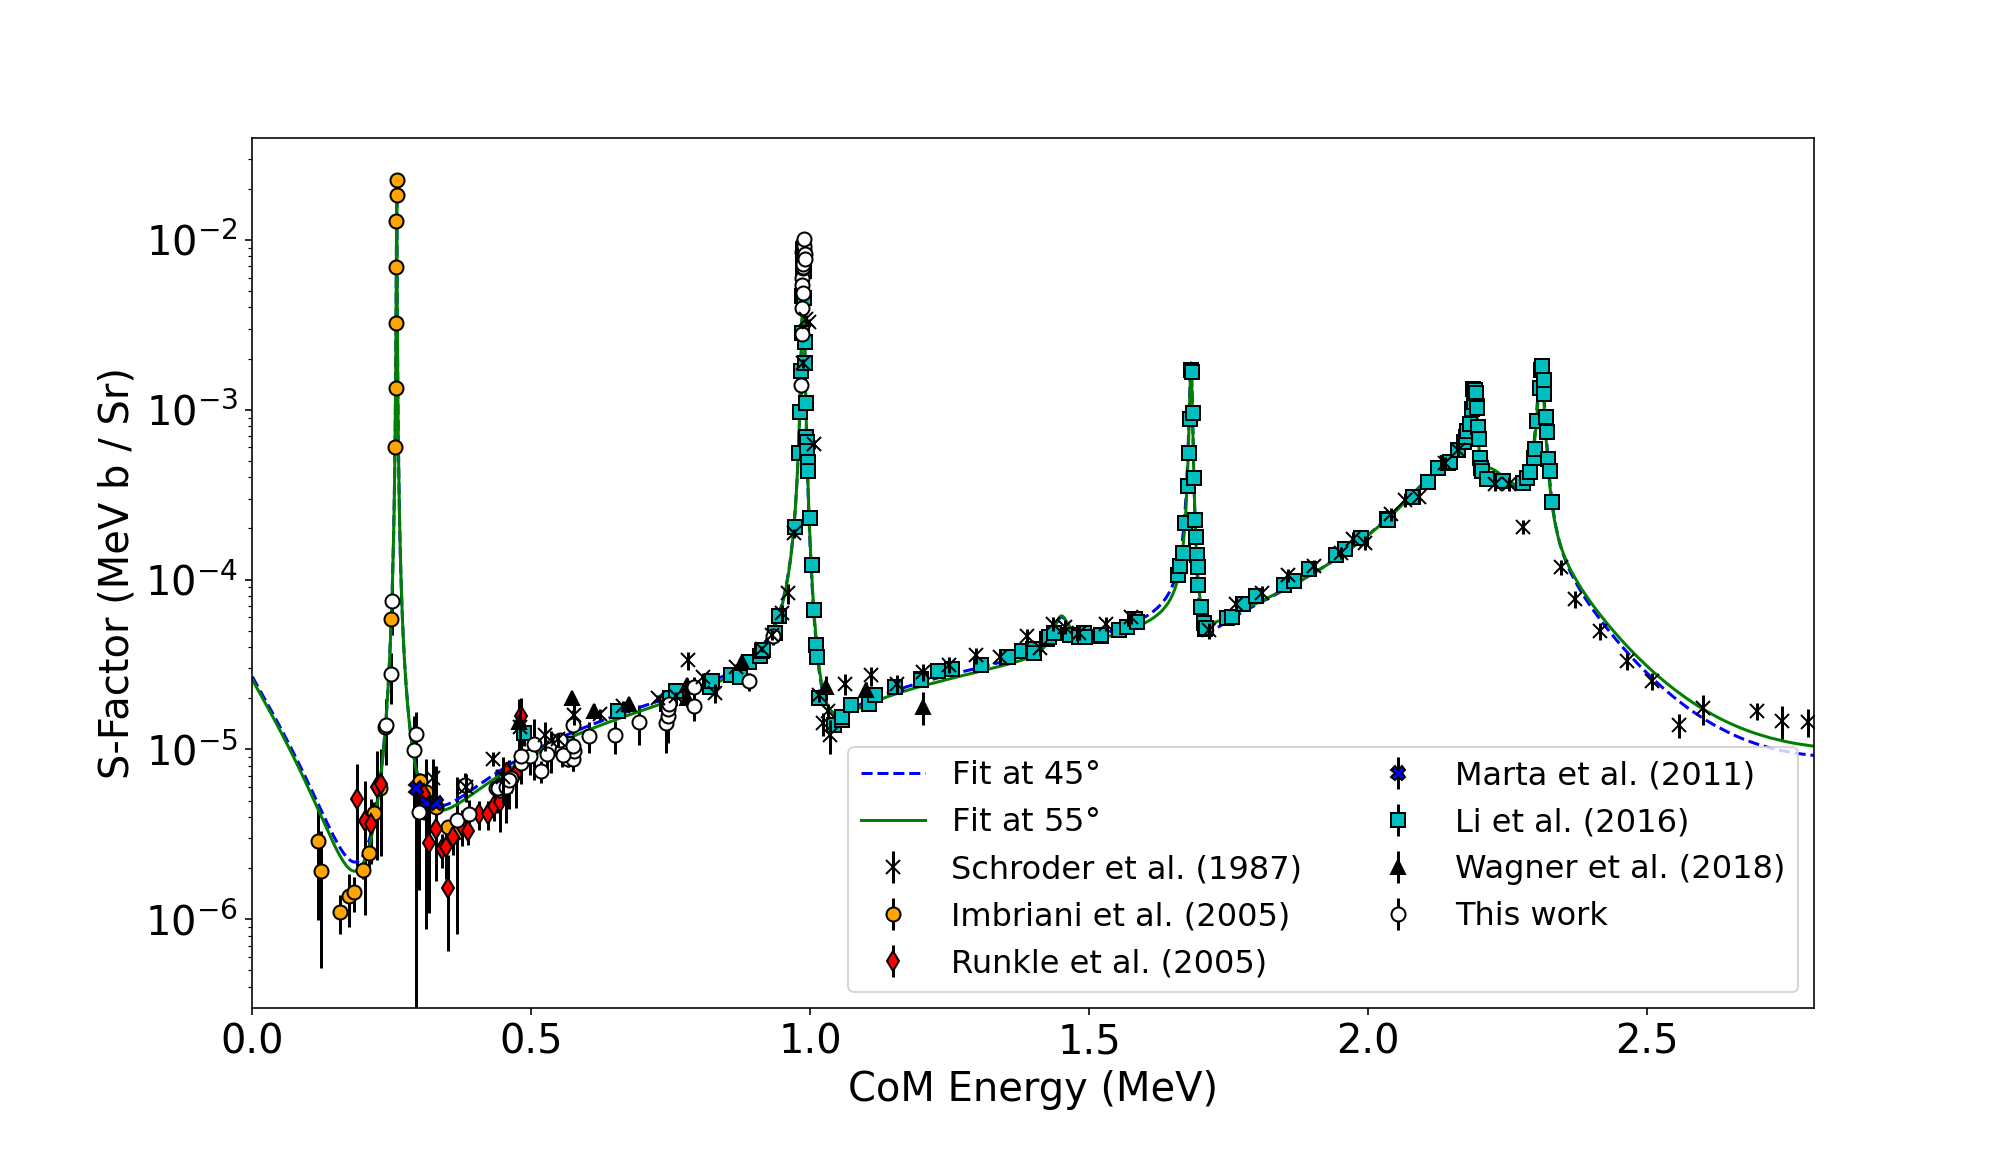
\includegraphics[width=1.0\columnwidth]{./figures/data_and_fits_whole.png}
\caption{$S$ factors for the R/DC $\rightarrow$ ground state transition for this work compared with those from Refs.~\cite{Imbriani2005, Marta2011, Runkle2005, Schroder1987, Li2016, Wagner2018} and extrapolated differential $S$-factor curves calculated with the \texttt{AZURE2} code. The data of \cite{Imbriani2005, Runkle2005, Marta2011, Wagner2018} have been scaled by a factor of $4\pi$ for the purposes of plotting the differential fits, but were treated an angle integrated when performing the fits. The data from \citet{Schroder1987} are corrected \cite{Adelberger2011} and then treated as differential (more detail in text). }
\label{fig: sfactor_best_fit}
\end{figure}

\begin{figure}
\centering
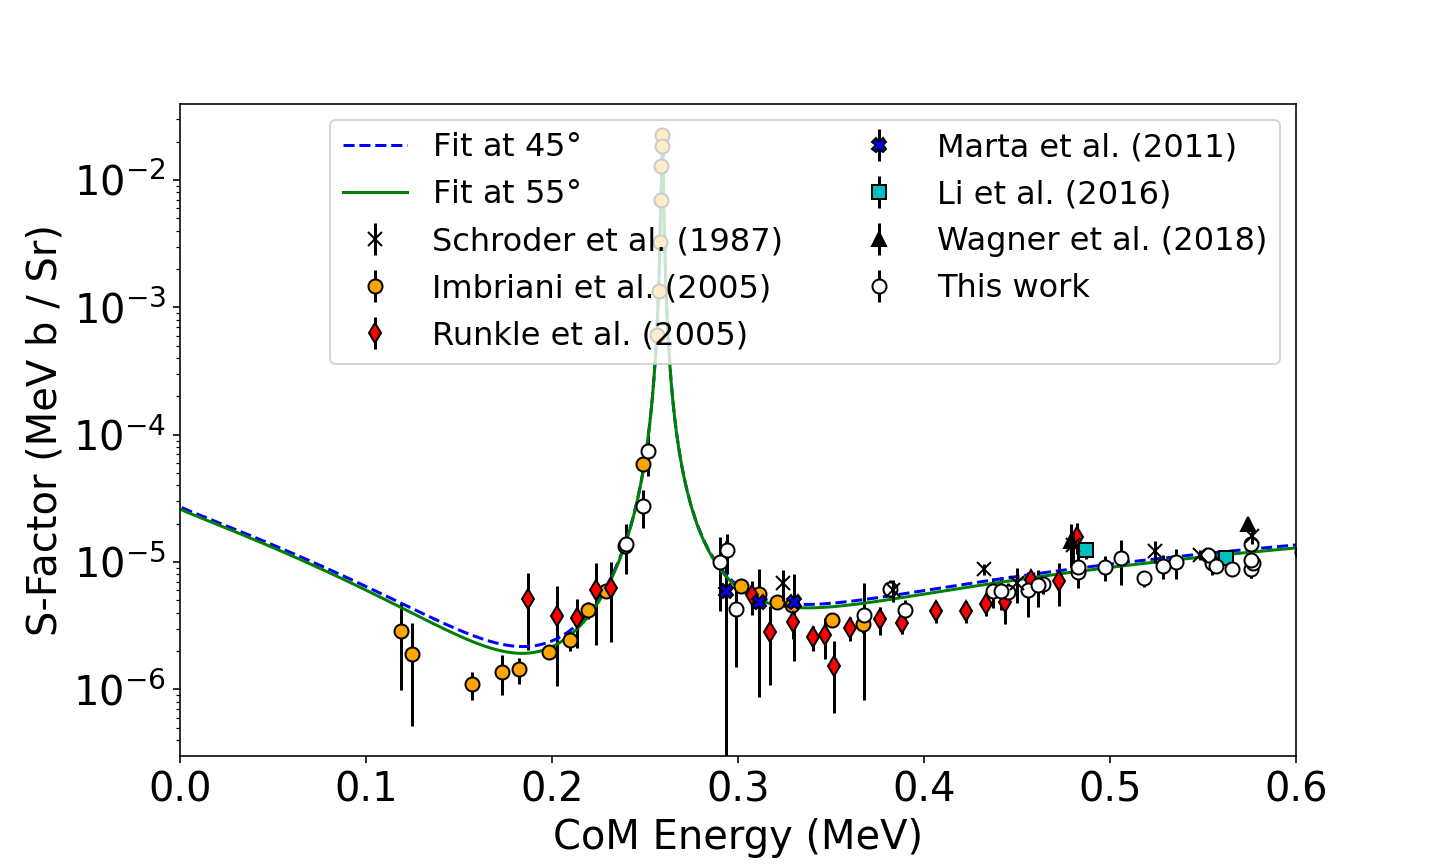
\includegraphics[width=1.0\columnwidth]{./figures/data_and_fits_low.png}
\caption{Low energy $S$-factor data and extrapolations for the R/DC $\rightarrow$ ground state transition for this work compared with those from Refs.~\cite{Imbriani2005, Marta2011, Runkle2005, Schroder1987, Li2016, Wagner2018} and extrapolated differential $S$-factor curves calculated with the \texttt{AZURE2} code. The data of \cite{Imbriani2005, Runkle2005, Marta2011, Wagner2018} have been scaled by a factor of $4\pi$ for the purposes of plotting the differential fits, but were treated an angle integrated when performing the fits. The data from \citet{Schroder1987} are corrected \cite{Adelberger2011} and then treated as differential (more detail in text). }
\label{fig: sfactor_best_low}
\end{figure}


The differential cross sections were investigated for the ways in which they are affected by different angles. The differential $S$-factor was calculated at four different angles, namely $0\degree$, $45\degree$, $55\degree$, and $135\degree$, based on the results of the best fit to the data. As can be seen in Fig.~\ref{fig: sfactor_differential_angles}, there are significant differences in the differential $S$-factor across the entire energy landscape. The fits at $45\degree$ and $55\degree$ are nearly identical. The fits at $0\degree$ and $135\degree$ exhibit the same behavior below the 278~keV resonance, and are notably larger. They are elevated immediately below the resonance, and while the gap decreases with energy, the extrapolated $S_{g.s.}(0)$ for the fits at $0\degree$ and $135\degree$ are approximately 15$\%$ higher than the extrapolations at $45\degree$ and $55\degree$. While reported as angle integrated, the low-energy data of \citet{Imbriani2005} and \citet{Runkle2005} were measured at $55\degree$ and $0\degree$ respectively, albeit, in very close geometry. As can be seen here, the discrepancy of these two data sets below the 278~keV resonance might be partly resolved by this effect. Specifically, a fit of these two datasets, and the respective differential fits at $0\degree$ and $55\degree$, are shown in Fig.~\ref{fig: sfactor_runkle_imbriani}. 


\begin{figure}
\centering
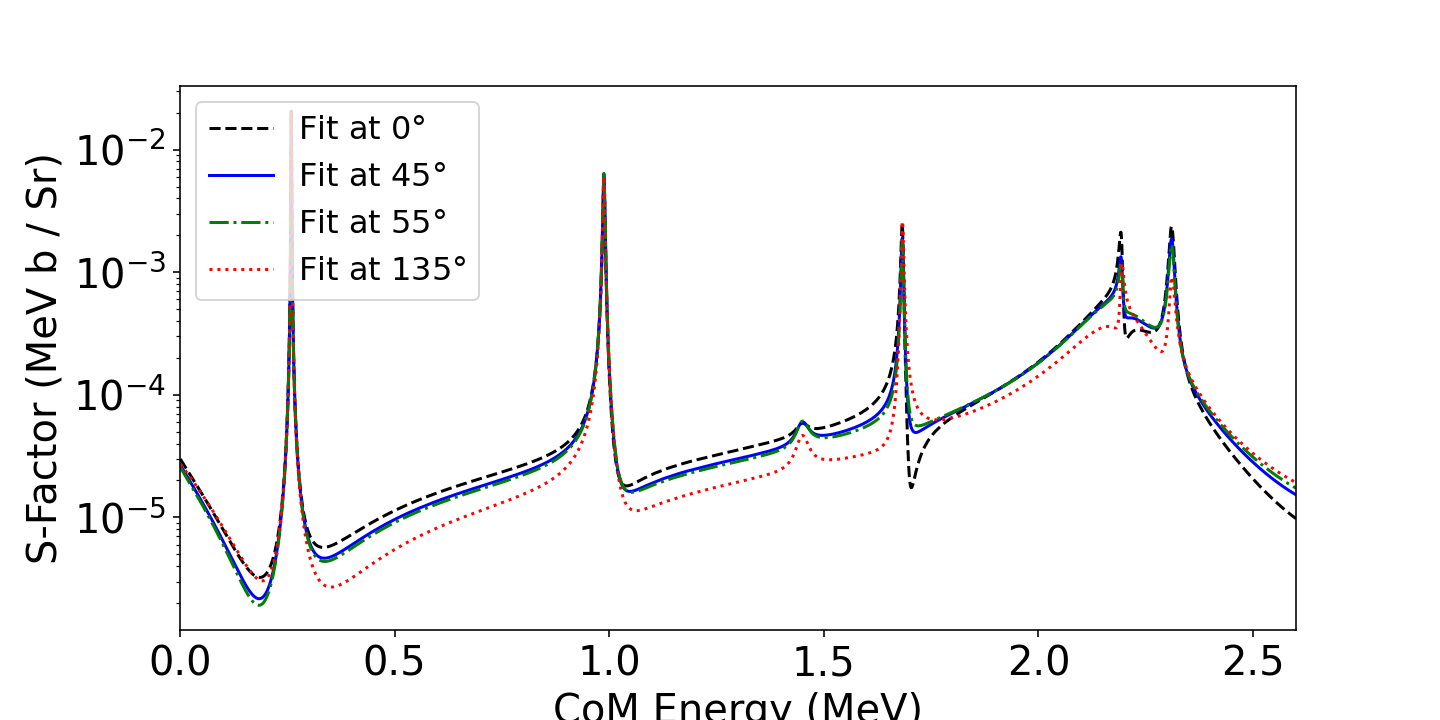
\includegraphics[width=1.0\columnwidth]{./figures/differential_fits.png}
\caption{Differential $S$ factors for the R/DC $\rightarrow$ ground state transition calculated from our best fit at $0\degree$, $45\degree$, $55\degree$, and $135\degree$. The behavior at different angles shows significant difference across the whole energy range for the reaction. }
\label{fig: sfactor_differential_angles}
\end{figure}

\begin{figure}
\centering
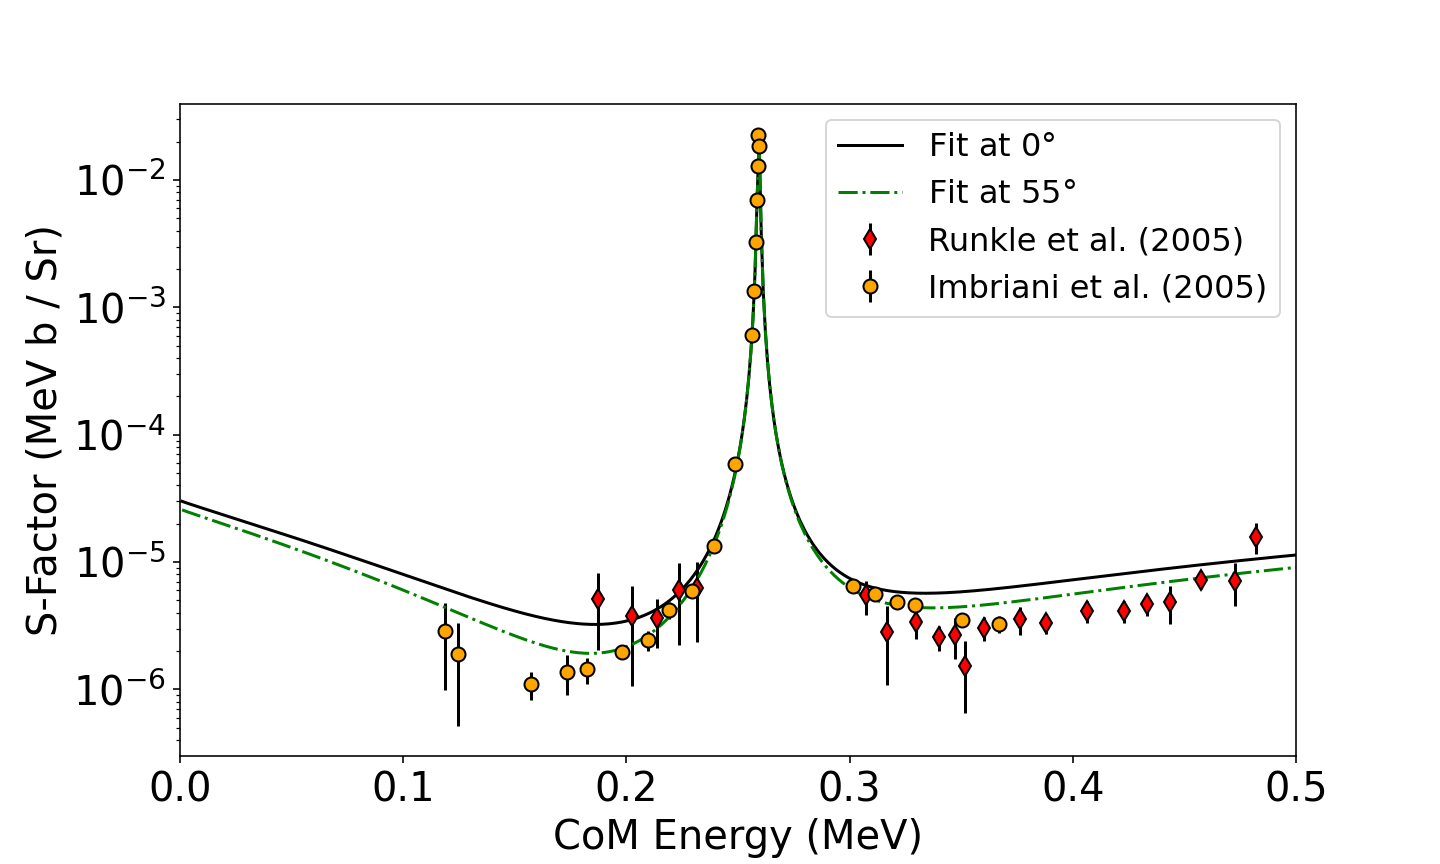
\includegraphics[width=1.0\columnwidth]{./figures/compare_runkle_imbriani.png}
\caption{$S$ factors for the R/DC $\rightarrow$ ground state transition from I\citet{Runkle2005} and \citet{Imbriani2005}, alongside the differential $S$-factors determined in this work at $0\degree$ and $55\degree$, respectively. The fits show significant differences in the behavior of the reaction below the resonance, where the large discrepancy between these datasets lie. The data have been scaled by a factor of $4\pi$ for the purposes of comparing to the differential fits, but were treated an angle integrated when performing the fits. }
\label{fig: sfactor_runkle_imbriani}
\end{figure}


For the capture to the excited state at 6.79 MeV, the present fit is in agreement with earlier investigations. The present extrapolated $S$-factor for this transition is $S_{6.79}(0) = 1.24 \pm 0.09$~keV~b. This agrees exactly with the recent measurement from \citet{Wagner2018} and simultaneously lies between those reported by \citet{Adelberger2011} and \citet{Li2016}, while agreeing with both with in their quoted uncertainties. 

For the capture to the ground state, the present result for the zero-energy extrapolated $S$-factor is $S_{g.s.}(0) = 0.33_{-0.08}^{+0.16} $~keV~b. This value is higher than either that of \citet{Wagner2018} ($0.19 \pm 0.05$ keV b), \citet{Adelberger2011} ($0.27 \pm 0.05$ keV b) or \citet{Imbriani2005} ($0.25 \pm 0.06$ keV b) while being lower than that reported by \citet{Li2016} ($0.42 \pm 0.04$(stat)$^{+0.09}_{-0.19}$(syst) keV b) and \citet{Runkle2005} ($0.49 \pm 0.08$ keV b). With these results for context, the current extrapolated value lies in the middle of the landscape of previous measurements. In addition, the data from the present measurement above the resonance agrees well with that from \citet{Runkle2005}, while the $R$-matrix fit overproduces the cross section over this energy range. This is not limited just to the present $R$-matrix fit. Most previous fits~\cite{PhysRevC.67.065804, Imbriani2005, Azuma2010, Adelberger2011, Li2016, Wagner2018} show a similar overproduction of the cross section in this energy region. 

The discrepancy between the ground state transition data sets (\citet{Imbriani2005} and \citet{Runkle2005}) and the $R$-matrix fit at low energies is reflected in the estimated uncertainty band of the low energy $S$ factor extrapolation. For the other 6.79~MeV transition, the data are in good agreement and a relative uncertainty in line with previous measurements was adopted. 

While this study does not report any measurements for the transition to the excited state at 6.17~MeV, a fit was performed, and an $S$-factor extrapolation was made, using the data from \citet{Schroder1987}, \citet{Runkle2005}, and \citet{Imbriani2005}. The present extrapolated $S$-factor for this transition is $S_{6.17}(0) = 0.12 \pm 0.04$~keV~b. This agrees well with the recently reported values of 0.12 in \citet{Azuma2010} and 0.13 $\pm$ 0.06 in \citet{Adelberger2011}.

With the above considertations, a new total $S$-factor for the $^{14}$N$(p,\gamma)^{15}$O reaction was calculated, giving a total $S$-factor of $S_{tot}(0) = 1.69 \pm 0.13$~keV~b. This value, as well as those for the individual transitions, are compared to literature values in Table \ref{table: new_s_factors}. The other transitions, not explicitly reported in this section, are expected to contribute less than $\sim5\%$ to the total low energy $S$-factor. 

This total $S$-factor, at zero-energy, is higher than those values reported in \cite{Imbriani2005, Marta2008, Adelberger2011} but agrees reasonably well within uncertainty and lies in near perfect agreement to the extrapolations reported in \cite{Runkle2005, Angulo2005}. This suggests a low-energy $S$-factor for the $^{14}$N$(p,\gamma)^{15}$O reaction, agreeing with the recent neutrino measurements by the Borexino group~\citet{agostini2020direct}, lies within the estimated uncertainty range. 


\begin{sidewaystable}[]
\caption{SUMMARY OF THE EXTRAPOLATED $S$-FACTORS}
\thisfloatpagestyle{plain}
\hspace*{-1.5cm}

\begin{threeparttable}
\begin{tabular}{@{}lllllll@{}}
\toprule
     &                                                          & \multicolumn{5}{c}{Astrophysical $S$-factor $S(0)$ (keV b)}                                                                                                                               \\ \midrule
Year & Reference                                                & R/DC $\rightarrow$ 0.00                         & R/DC $\rightarrow$ 6.79                 & R/DC $\rightarrow$ 6.17        & Others$^{d}$ & Total                                         \\
\hline
1987 & Schr{\"o}der \textit{et al.} \cite{Schroder1987}          & 1.55 $\pm$ 0.34                                 & 1.41 $\pm$ 0.02                         & 0.14 $\pm$ 0.05                & 0.1          & 3.20 $\pm$ 0.54                               \\
2001 & Angulo \textit{et al.}$^{a}$ \cite{Angulo2001}            & 0.08$^{+0.13}_{-0.06}$                          & 1.63 $\pm$ 0.17                         & 0.06$^{+0.01}_{-0.02}$          & $--$         & 1.77 $\pm$ 0.20                               \\
2003 & Mukhamedzhanov \textit{et al.} \cite{Mukhamedzhanov2003} & 0.15 $\pm$ 0.07                                 & 1.40 $\pm$ 0.20                         & 0.133 $\pm$ 0.02               & 0.02         & 1.70 $\pm$ 0.22                               \\
2004 & Formicola \textit{et al.} \cite{Formicola2004}            & 0.25 $\pm$ 0.06                                 & 1.35 $\pm$ 0.05 (stat) & 0.06$^{+0.01 \text{b}}_{-0.02}$ & 0.04         & 1.7 $\pm$ 0.1 (stat)        \\
 & & & $\pm$ 0.08 (sys) & & & $\pm$ 0.02 (sys) \\
2005 & Imbriani \textit{et al.} \cite{Imbriani2005}              & 0.25 $\pm$ 0.06                                 & 1.21 $\pm$ 0.05                         & 0.08 $\pm$ 0.03                & 0.07         & 1.61 $\pm$ 0.08                               \\
2005 & Runkle \textit{et al.} \cite{Runkle2005}                  & 0.49 $\pm$ 0.08                                 & 1.15 $\pm$ 0.05                         & 0.04 $\pm$ 0.01                & $--$         & 1.68 $\pm$ 0.09                               \\
2005 & Angulo \textit{et al.} \cite{Angulo2005}                  & 0.25 $\pm$ 0.08                                 & 1.35 $\pm$ 0.04                         & 0.06 $\pm$ 0.02                & 0.04         & 1.70 $\pm$ 0.07 (stat)       \\
 & & & & & & $\pm$ 0.10 (sys) \\
2006 & Bemmerer \textit{et al.} \cite{Bemmerer2006}              & $--$                                            & $--$                                    & $--$                           & $--$         & 1.74 $\pm$ 0.14 (stat)  \\
 & & & & & & $\pm$ 0.14 (sys)$^{c}$ \\
2008 & Marta \textit{et al.} \cite{Marta2008}                    & 0.20 $\pm$ 0.05                                 & $--$                                    & 0.09 $\pm$ 0.07                & $--$         & 1.57 $\pm$ 0.13                               \\
2010 & Azuma \textit{et al.} \cite{Azuma2010}                    & 0.28                                            & 1.3                                     & 0.12                           & 0.11         & 1.81                                          \\
2011 & Adelberger \textit{et al.} \cite{Adelberger2011}          & 0.27 $\pm$ 0.05                                 & 1.18 $\pm$ 0.05                         & 0.13 $\pm$ 0.06                & 0.08         & 1.66 $\pm$ 0.08                               \\
2016 & Li \textit{et al.} \cite{Li2016}                          & 0.42 $\pm$ 0.04 (stat)   & 1.29 $\pm$ 0.06 (stat)  & $--$                           & $--$         & $--$                                          \\
 & & $^{+0.09}_{-0.19}$(sys) & $\pm$ 0.06 (sys) & & & \\
2018 & Wagner \textit{et al.} \cite{Wagner2018}                  & 0.19 $\pm$ 0.01 (stat)          & 1.24 $\pm$ 0.02 (stat) & $--$                           & $--$         & $--$                                          \\
 & & $\pm$ 0.05 (sys) &  $\pm$ 0.11 (sys)  & & & \\ 
2021 & This work                  & $0.33_{-0.08}^{+0.16} $           & 1.24 $\pm$ 0.09  &  0.12 $\pm$ 0.04$^{d}$              & $--$         & 1.69 $\pm$ 0.13 \\
 \bottomrule
\end{tabular}
\begin{tablenotes}
\small 
\item A summary of reported $S$-factors, including this work. a) $R$-matrix analysis on available data, not a measurement. b) Adopted from Angulo \textit{et al.} \cite{Angulo2001}. c) Measured $S$-factor at 70 keV. d) Calculated difference of the total $S(0)$ from the other transitions. d) Fit to the data of \cite{Schroder1987, Runkle2005, Imbriani2005} as no new data for this transition was measured.
\end{tablenotes}
\end{threeparttable}
\label{table: new_s_factors}
\end{sidewaystable}




\section{Reaction rates}
\label{sec: reaction rates}


For the transitions reported here, the reaction rates were calculated with \texttt{AZURE2} for the temperature range of 0.001 GK to 10 GK with 2000 steps spaced equally in $\log(T_{9})$. Like the $S$-factors, the reaction rate contributions from the ground state and 6.79~MeV transitions were calculated from our data in tandem with the literature data of Refs.~\cite{Formicola2004, Imbriani2005, Marta2008, Marta2011, Runkle2005, Schroder1987, Li2016, Wagner2018}, while the contribution from the 6.17~MeV transition was calculated exclusively from the literature data of Refs.~\cite{Runkle2005, Imbriani2005, Schroder1987}. Finally, the remainder of the strength from the $E_{x}= 7.556$~MeV from other transitions is added to the reaction rate using the narrow resonance approximation.

The results for the reaction rates are given in Table~\ref{table: reaction_rates} compared with those from \citet{Caughlan1988}, \citet{Angulo1999}, and \citet{Imbriani2005} in Fig.~\ref{fig: rrate_comp}. At lower temperatures, the present rate is approximately 15$\%$ higher than those published by \citet{Imbriani2005}, while the present rates are lower than the other two reported values. It be considered that the calculations of \citet{Caughlan1988} and \citet{Angulo1999} are based only on the uncorrected data from \citet{Schroder1987}. 


\begin{sidewaystable}[]
\thisfloatpagestyle{plain}
\caption{REACTION RATES FOR $^{14}$N$(p,\gamma)^{15}$O }
\begin{center}
\begin{threeparttable}
\begin{tabular}{@{}lllllllll@{}}
\toprule
$T_{9}$       & R/DC $\rightarrow$ 0.00 & R/DC $\rightarrow$ 5.18* & R/DC $\rightarrow$ 6.17 & R/DC $\rightarrow$ 6.79 & Total (this work) & Total \cite{Caughlan1988} & Total \cite{Angulo1999} & Total \cite{Imbriani2005} \\ \midrule
1.00E-03 & 4.92E-58                & 0.00E+00                 & 1.97E-58                & 1.96E-57                & 2.65E-57          & 4.58E-57                  & 5.40E-57                & 2.33E-57                  \\
1.50E-03 & 8.05E-50                & 0.00E+00                 & 3.29E-50                & 3.27E-49                & 4.40E-49          & 7.63E-49                  & 8.97E-49                & 3.90E-49                  \\
2.00E-03 & 1.35E-44                & 0.00E+00                 & 5.63E-45                & 5.54E-44                & 7.45E-44          & 1.30E-43                  & 1.52E-43                & 6.66E-44                  \\
3.01E-03 & 4.10E-38                & 0.00E+00                 & 1.78E-38                & 1.73E-37                & 2.32E-37          & 4.06E-37                  & 4.72E-37                & 2.09E-37                  \\
4.00E-03 & 4.68E-34                & 0.00E+00                 & 2.10E-34                & 2.02E-33                & 2.70E-33          & 4.74E-33                  & 5.49E-33                & 2.46E-33                  \\
5.01E-03 & 4.05E-31                & 3.58E-255                & 1.88E-31                & 1.79E-30                & 2.38E-30          & 4.19E-30                  & 4.83E-30                & 2.18E-30                  \\
7.52E-03 & 2.19E-26                & 1.17E-168                & 1.09E-26                & 1.02E-25                & 1.35E-25          & 2.38E-25                  & 2.72E-25                & 1.24E-25                  \\
1.00E-02 & 1.98E-23                & 1.05E-125                & 1.05E-23                & 9.58E-23                & 1.26E-22          & 2.24E-22                  & 2.54E-22                & 1.17E-22                  \\
1.50E-02 & 1.03E-19                & 1.78E-82                 & 6.16E-20                & 5.41E-19                & 7.06E-19          & 1.26E-18                  & 1.42E-18                & 6.63E-19                  \\
2.00E-02 & 2.30E-17                & 9.58E-61                 & 1.54E-17                & 1.30E-16                & 1.68E-16          & 3.03E-16                  & 3.37E-16                & 1.59E-16                  \\
3.01E-02 & 1.80E-14                & 2.60E-39                 & 1.47E-14                & 1.16E-13                & 1.49E-13          & 2.69E-13                  & 2.95E-13                & 1.41E-13                  \\
4.00E-02 & 1.11E-12                & 1.03E-28                 & 1.09E-12                & 8.05E-12                & 1.03E-11          & 1.87E-11                  & 2.03E-11                & 9.81E-12                  \\
4.99E-02 & 2.00E-11                & 2.20E-22                 & 2.34E-11                & 1.62E-10                & 2.05E-10          & 3.76E-10                  & 4.05E-10                & 1.98E-10                  \\
7.52E-02 & 2.26E-09                & 7.49E-14                 & 4.08E-09                & 2.39E-08                & 3.02E-08          & 5.52E-08                  & 5.84E-08                & 2.95E-08                  \\
1.00E-01 & 3.87E-08                & 1.01E-09                 & 1.11E-07                & 5.19E-07                & 6.70E-07          & 1.20E-06                  & 1.25E-06                & 6.68E-07                  \\
1.50E-01 & 2.38E-06                & 1.22E-05                 & 5.66E-05                & 4.06E-05                & 1.12E-04          & 1.29E-04                  & 1.35E-04                & 1.10E-04                  \\
2.00E-01 & 1.26E-04                & 1.23E-03                 & 4.99E-03                & 1.86E-03                & 8.21E-03          & 8.34E-03                  & 8.54E-03                & 7.87E-03                  \\
3.01E-01 & 9.48E-03                & 9.92E-02                 & 3.94E-01                & 1.32E-01                & 6.35E-01          & 6.61E-01                  & 6.55E-01                & 6.03E-01                  \\
4.00E-01 & 7.41E-02                & 7.74E-01                 & 3.07E+00                & 1.03E+00                & 4.95E+00          & 5.21E+00                  & 5.12E+00                & 4.68E+00                  \\
4.99E-01 & 2.38E-01                & 2.47E+00                 & 9.80E+00                & 3.30E+00                & 1.58E+01          & 1.66E+01                  & 1.63E+01                & 1.50E+01                  \\
7.52E-01 & 1.05E+00                & 1.01E+01                 & 4.03E+01                & 1.41E+01                & 6.56E+01          & 6.71E+01                  & 6.71E+01                & 6.24E+01                  \\
1.00E+00 & 2.41E+00                & 1.78E+01                 & 7.11E+01                & 2.69E+01                & 1.18E+02          & 1.18E+02                  & 1.19E+02                & 1.12E+02                  \\
1.50E+00 & 1.32E+01                & 2.64E+01                 & 1.06E+02                & 5.29E+01                & 1.98E+02          & 2.02E+02                  & 1.92E+02                & 1.88E+02                  \\
2.00E+00 & 4.88E+01                & 2.83E+01                 & 1.15E+02                & 8.57E+01                & 2.78E+02          & 3.12E+02                  & 2.69E+02                & 2.43E+02                  \\
3.01E+00 & 2.28E+02                & 2.54E+01                 & 1.10E+02                & 1.87E+02                & 5.50E+02          & 7.46E+02                  & 5.91E+02                & 3.28E+02                  \\
4.00E+00 & 5.74E+02                & 2.12E+01                 & 1.02E+02                & 3.33E+02                & 1.03E+03          & 1.46E+03                  & 1.20E+03                & 3.98E+02                  \\
4.99E+00 & 1.06E+03                & 1.77E+01                 & 9.85E+01                & 5.12E+02                & 1.69E+03          & 2.35E+03                  & 2.06E+03                & 4.57E+02                  \\
7.52E+00 & 2.51E+03                & 1.17E+01                 & 9.90E+01                & 1.07E+03                & 3.69E+03          & 4.45E+03                  & 4.81E+03                & 5.75E+02                  \\
9.95E+00 & 3.78E+03                & 8.47E+00                 & 1.07E+02                & 1.64E+03                & 5.54E+03          & 6.23E+03                  & 7.10E+03                & 6.55E+02                  \\ \bottomrule
\end{tabular}
\begin{tablenotes}
\small 
\item * Contribution added using the narrow resonance approximation.
\end{tablenotes}
\end{threeparttable}
\label{table: reaction_rates}
\end{center}
\end{sidewaystable}


\begin{figure}[htbp]
\centering
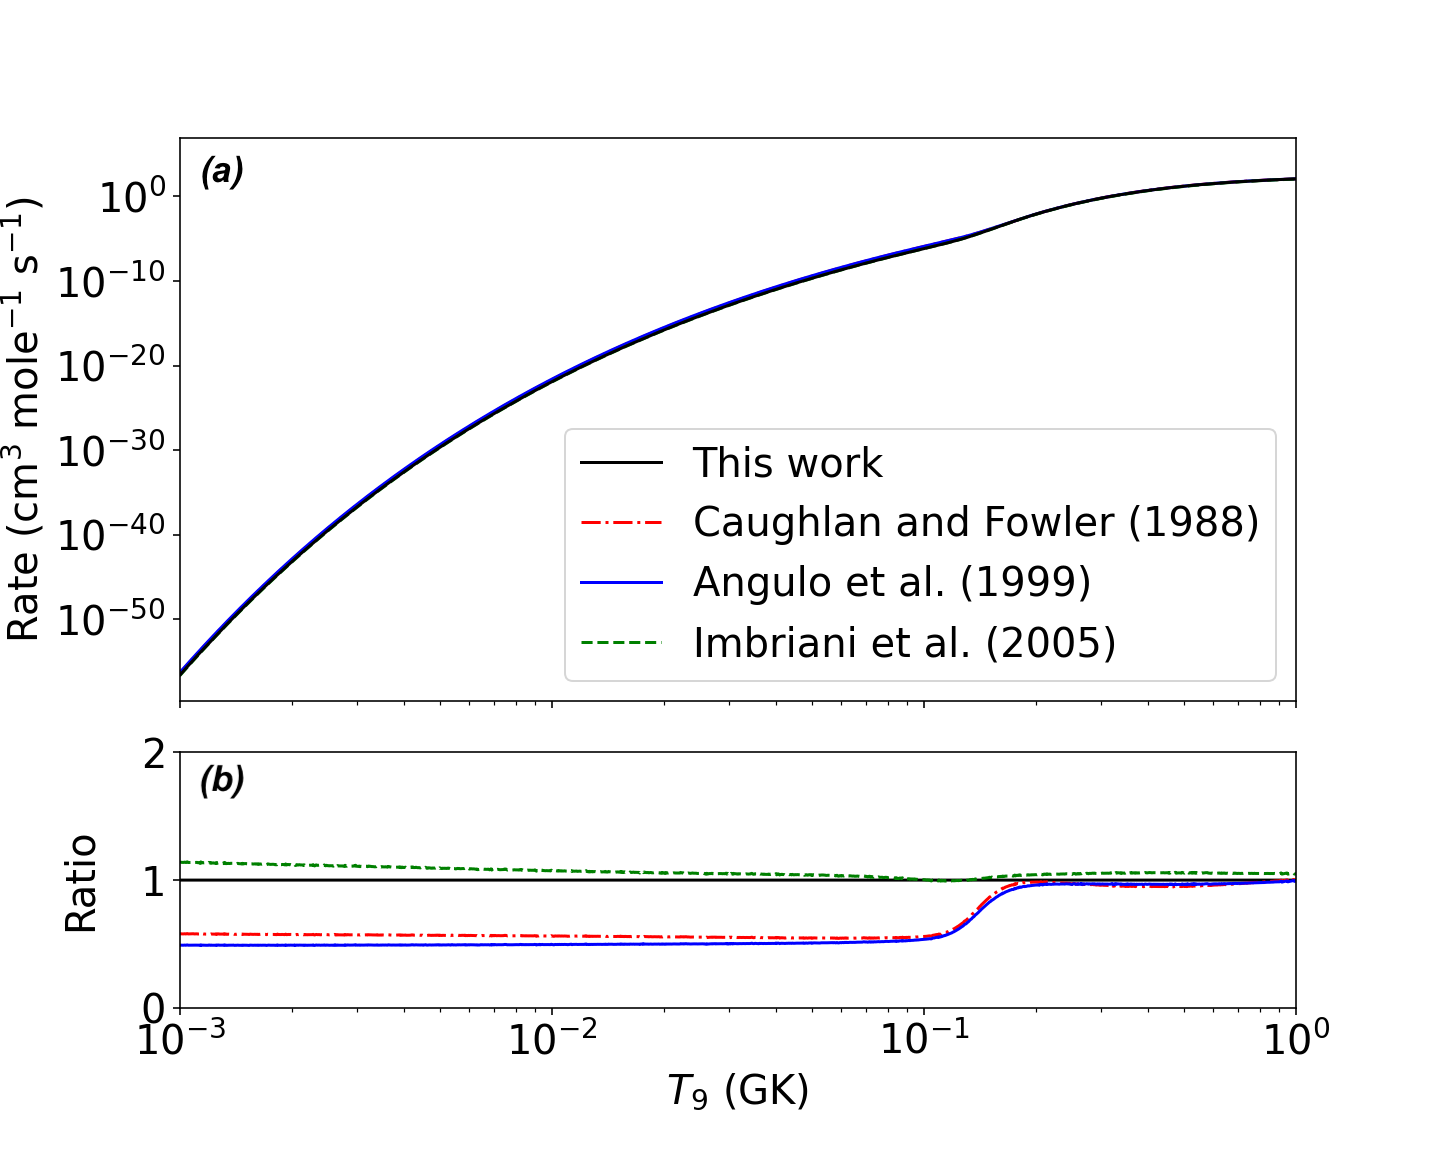
\includegraphics[width=1.0\columnwidth]{./figures/rr_with_518_zoom.png}
\caption{The reaction rate from the present work compared with the rates presented in \citet{Caughlan1988}, \citet{Angulo1999}, and \citet{Imbriani2005}. The rates in this work were calculated numerically with the \texttt{AZURE2} software. a) Reaction rates given in cm$^{3}$ mole$^{-1}$ s$^{-1}$. b) Ratio of the present rate to the given literature rates. The rise at approximately 0.1 GK corresponds to the contribution from the transition to the 5.18 MeV excited state out of the $E_{x}= 7.556$ MeV resonance. }
\label{fig: rrate_comp}
\end{figure}

Ultimately, the present higher zero-energy $S$-factors translate to a higher reaction rate at stellar temperatures, indicating an agreement with the results presented by the Borexino group \cite{agostini2020direct}.


% % uncomment the following lines,
% if using chapter-wise bibliography
%
% \bibliographystyle{ndnatbib}
% \bibliography{example}
